 
\chapter{Sets}
\label{ch:sets}

{\em No more turkey, but I'd like some more of the bread it ate. --Hank Ketcham}


\section{Basic notions of set theory}
\label{sec:basic_set_notions}

In modern mathematics there is an area called \index{Category theory} 
Category theory\footnote{The classic text by Saunders Mac Lane \cite{macl} %
is still considered one of the best introductions to Category theory.} 
which studies the 
relationships between different areas of mathematics.  More precisely,
the founders of category theory noticed that essentially the same theorems 
and proofs could be found in many different mathematical fields -- with
only the names of the structures involved changed.  In this sort of
situation one can make what is known as a \emph{categorical} argument
in which one proves the desired result in the abstract, without reference
to the details of any particular field.  In effect this allows one
to prove many theorems at once -- all you need to convert an abstract
categorical proof into a concrete one relevant to a particular area
is a sort of key or lexicon to provide the correct names for things.
Now, category theory probably shouldn't really be studied until you 
have a background that includes enough different fields that you can
make sense of their categorical correspondences.  Also, there are 
a good many mathematicians who deride category theory as 
``abstract nonsense.''   But, as someone interested in developing a facility
with proofs, you should be on the lookout for categorical correspondences.
If you ever hear yourself utter something like ``well, the proof of 
\emph{that} goes just like the proof of the 
(insert weird technical-sounding name here) theorem'' you are  
probably noticing a categorical correspondence.  

Okay, so category theory won't be of much
use to you until much later in your mathematical career (if at all), and 
one could argue that it doesn't really save that much effort.  Why not just do two or three different 
proofs instead of learning a whole new field so we can combine 
them into one?  Nevertheless, category theory is being
mentioned here at the beginning of the chapter on sets.  Why? 

We are about to see our first example of a categorical correspondence.
Logic and Set theory are different aspects of the same thing.  To
describe a set people often quote 
\index{G\"{o}del, Kurt} Kurt G\"{o}del -- 
``A set is a Many that allows itself to be thought of as a One.''  (Note
how the attempt at defining what is really an elemental, undefinable
concept ends up sounding rather mystical.)  A more practical approach is
to think of a set as the collection of things that make some open sentence
\emph{true}.\footnote{This may sound less metaphysical,
but this statement is also faulty because it defines ``set'' in terms of ``collection'' -- which will of course be defined elsewhere as ``the sort of things of which sets are one example.''} 

Recall that in Logic the atomic concepts were ``true'', ``false'', 
``sentence'' and ``statement.''    In Set theory, they are ``set'', 
``element'' and ``membership.''  These concepts (more or less) correspond to
one another.  In most books, a set is denoted either using the letter $M$ 
(which stands for the German word ``menge'') or early alphabet capital roman 
letters --
$A$, $B$, $C$, \emph{et cetera}.  Here, we will often emphasize the connection between
sets and open sentences in Logic by using a subscript notation.  The set that
corresponds to the open sentence $P(x)$ will be denoted $S_P$, we call
$S_P$ the \index{truth set} \emph{truth set} of~$P(x)$. 

\[ S_P = \{ x \suchthat P(x) \} \]


On the other hand, when we have a set given in the absence of any open 
sentence, we'll be happy to use the early alphabet, capital roman letters 
convention -- or frankly, any other letters we feel like!
Whenever we have a set $A$ given, it is easy to state a logical 
open sentence that would correspond to it.  The membership question: $M_A(x) =
\,$ ``Is $x$ in the set $A$?''  Or, more succinctly, 
$M_A(x) = \,$ ``$x \in A$''.   Thus the atomic concept ``true'' from Logic
corresponds to the answer ``yes'' to the membership question in Set theory
(and of course ``false'' corresponds to ``no'').

There are many interesting foundational issues which we are going to
sidestep in our current development of Set theory.  For instance,
recall that in Logic we always worked inside some 
\index{universe of discourse}``universe of discourse.''
As a consequence of the approach we are taking now, all of our set theoretic
work will be done within some unknown 
\index{universal set}``universal'' set.  Attempts at 
specifying (\emph{a priori}) a universal set for doing mathematics within 
are doomed to failure.  In the early days of the twentieth century
they attempted to at least get Set theory itself on a firm footing by
defining the universal set to be ``the set of all sets'' -- an innocuous
sounding idea that had funny consequences (we'll investigate this in 
Section~\ref{sec:russell}).  

In Logic we had ``sentences'' and ``statements,'' the latter were 
distinguished as having definite truth values.  The corresponding
thing in Set theory is that sets have the property that we can always
tell whether a given object is or is not in them.  If it ever becomes
necessary to talk about ``sets'' where we're not really sure what's in
them we'll use the term \emph{collection}.
  
You should think of a set as being an \emph{unordered} collection of 
things, thus $\{ \mbox{popover}, 1, \mbox{froggy} \}$ and  
$\{ 1, \mbox{froggy}, \mbox{popover} \}$ are two ways to represent the 
same set.  Also, a set either contains, or doesn't contain, a given element.
It doesn't make sense to have an element in a set multiple times.  By
convention, if an element is listed more than once when a set is
listed  we ignore the repetitions.  So, the sets
$\{ 1, 1\}$ and $\{1\}$ are really the same thing.  If the notion
of a set containing multiple instances of its elements is needed there
is a concept known as a 
\index{multiset}\emph{multiset} that is studied in Combinatorics.
In a multiset, each element is preceded by a so-called 
\index{repetition number}\emph{repetition number}
which may be the special symbol $\infty$ (indicating an unlimited number
of repetitions).  The multiset concept is useful when studying puzzles like
``How many ways can the letters of MISSISSIPPI be rearranged?'' because the
letters in MISSISSIPPI can be expressed as the multiset $\{1\cdot M, 4\cdot I,
2\cdot P, 4\cdot S \}$.  With the exception of the following exercise, in the
remainder of this chapter we will only be concerned with sets, never multisets.

\begin{exer}
(Not for the timid!) How many ways can the letters of MISSISSIPPI be arranged?
\end{exer}

If a computer scientist were seeking a data structure to implement the
notion of ``set,'' he'd want a sorted list where repetitions of an entry
were somehow disallowed.  We've already noted that a set should be thought of
as an unordered collection, and yet it's been asserted that a \emph{sorted}
list would be the right vehicle for representing a set on a computer.  Why?
One reason is that we'd like to be able to tell (quickly) whether two sets
are the same or not.  If the elements have been presorted it's easier.

Consider the difficulty in deciding whether the following two sets are
equal.

\vfill

\[ S_1 = \{ \spadesuit, 1, e, \pi, \diamondsuit, A, \Omega, h, \oplus, \epsilon \} \]

\vfill

\[ S_2 = \{ A, 1, \epsilon, \pi, e, s, \oplus,  \spadesuit, \Omega, \diamondsuit \} \]

\newpage
If instead we compare them after they've been sorted, the job is much easier.

\[ S_1 = \{1, A, \diamondsuit, e, \epsilon, h, \Omega, \oplus, \pi, \spadesuit \} \]

\[ S_2 = \{1, A, \diamondsuit, e, \epsilon, \Omega, \oplus, \pi, s, \spadesuit \} \]

This business about ordered versus unordered comes up fairly often so it's 
worth investing a few moments to figure out how it works.  If a collection
of things that is inherently unordered is handed to us we generally \emph{put}
them in an order that is pleasing to us.  Consider receiving five cards
from the dealer in a card game, or extracting seven letters from the bag 
in a game of Scrabble.  If, on the other hand, we receive 
a collection where order
is important we certainly \emph{may not} rearrange them.  Imagine someone
receiving the telephone number of an attractive other but writing it down
with the digits sorted in increasing order!  

\begin{exer}
Consider a universe consisting of just the first 5 natural numbers
$U = \{ 1, 2, 3, 4, 5 \}$.  How many different sets having 4 elements
are there in this universe?  How many different ordered collections of 4 
elements are there? 
\end{exer}

The last exercise suggests an interesting question.  If you have 
a universal set of some fixed (finite) size, how many different sets
are there?  Obviously you can't have any more elements in a set than
are in your universe.  What's the smallest possible size for a set?
Many people would answer 1 -- which isn't unreasonable! -- after all
a set is supposed to be a collection of things, and is it really possible
to have a \emph{collection} with nothing in it?  The standard answer is
0 however, mostly because it makes a certain counting formula work out
nicely.  A set with one element is known as a 
\index{singleton set}\emph{singleton set} 
(note the use of the indefinite article).  A set with no elements
is known as the 
\index{empty set}\emph{empty set} (note the definite article).  There
are as many singletons as there are elements in your universe.  They
aren't the same though, for example $1 \neq \{ 1 \}$.  There is 
only one empty set and it is denoted $\emptyset$ -- irrespective of the
universe we are working in.

Let's have a look at a small example.  Suppose we have a universal set
with 3 elements, without loss of generality, $\{1, 2, 3\}$.  It's 
possible to construct a set, whose elements are all the possible sets
in this universe.  This set is known as the 
\index{power set}\emph{power set} of the universal
set.  Indeed, we can construct the power set of \emph{any} set $A$ and
we denote it with the symbol ${\mathcal P}(A)$.  Returning to our
example we have 

\begin{center}
\begin{tabular}{rcl}
 ${\mathcal P}(\{1, 2, 3 \}) = $ & $\left\{ \rule{0pt}{10pt}  \right.$ & $\emptyset,$ \\
  & & $\{ 1 \},  \{ 2 \},  \{ 3 \},$ \\
  & & $\{ 1, 2 \},  \{ 1, 3 \},  \{ 2, 3 \},$ \\
  & & $\left.   \{ 1, 2, 3 \} \rule{0pt}{10pt} \right\}.$
\end{tabular}
\end{center}

\begin{exer} \rule{0pt}{0pt}

Find the power sets $ {\mathcal P}(\{1, 2 \})$ and 
${\mathcal P}(\{1, 2, 3, 4 \})$.  

Conjecture a formula for the number 
of elements (these are, of course, \emph{sets}) in 
${\mathcal P}(\{1, 2, \ldots n \})$.

Hint: If your conjectured formula is correct you should see 
why these sets are named as they are. 

\end{exer}

One last thing before we end this section.  The size (a.k.a. \index{cardinality}cardinality) of a set is just the number of elements in it.  We use the
very same symbol for cardinality as we do for the absolute value of a
numerical entity.  There should really never be any confusion.  If $A$ is
a set then $|A|$ means that we should count how many things are in $A$.
If $A$ isn't a set then we are talking about the ordinary absolute value

\clearpage 

\noindent{\large \bf Exercises --- \thesection\ }

\begin{enumerate}
\item What is the power set of $\emptyset$?  Hint: if you got the last exercise
in the chapter you'd know that this power set has $2^0 = 1$ element.

\hint{The power set of a set always includes the empty set as well as the whole set that we
are forming the power set of.  In this case they happen to coincide so ${\mathcal P}(\emptyset) = \{ \emptyset \}$.  Notice that $2^0 =1$.}

\item Try iterating the power set operator.  What is ${\mathcal P}({\mathcal P}(\emptyset))$?  What is ${\mathcal P}({\mathcal P}({\mathcal P}(\emptyset)))$?

\hint{I won't spoil you're fun, but as a check ${\mathcal P}({\mathcal P}(\emptyset))$ should have $2$ elements, and ${\mathcal P}({\mathcal P}({\mathcal P}(\emptyset)))$ should have $4$.}

\item Determine the following cardinalities.
  \begin{enumerate}
    \item $A = \{ 1, 2, \{3, 4, 5\}\} \quad |A| = $\rule{36pt}{1pt}
    \item $B = \{ \{1, 2, 3, 4, 5\} \} \quad |B| = $\rule{36pt}{1pt}  
  \end{enumerate}

\hint{Three and one}

\item What, in Logic, corresponds the notion $\emptyset$ in Set theory?

\hint{A contradiction.}

\item What, in Set theory, corresponds to the notion $t$ (a tautology) in Logic?

\hint{The universe of discourse.}

\item What is the truth set of the proposition $P(x) = $ ``3 divides $x$ and 2 divides $x$''?

\hint{ The set of all multiples of $6$.}

\item Find a logical open sentence such that $\{0, 1, 4, 9, \ldots \}$ is
its truth set.

\hint{Many answers are possible.  Perhaps the easiest is $\exists y \in \Integers, x = y^2$.}

\item How many singleton sets are there in the power set of 
$\{a,b,c,d,e\}$?  ``Doubleton'' sets?

\hint{5, 10}

\item How many 8 element subsets are there in
\[ {\mathcal P}(\{a,b,c,d,e,f,g,h,i,j,k,l,m,n,o,p\})? \]

\hint{ $\binom{16}{8} = 12870$}

\item How many singleton sets are there in the power set of 
$\{1,2,3, \ldots n\}$?

\hint{$n$}

\end{enumerate}



%% Emacs customization
%% 
%% Local Variables: ***
%% TeX-master: "GIAM-hw.tex" ***
%% comment-column:0 ***
%% comment-start: "%% "  ***
%% comment-end:"***" ***
%% End: ***



\newpage

\section{Containment}
\label{sec:cont}

There are two notions of being ``inside'' a set.  A thing may be
an \emph{element} of a set, or may be contained as
a subset.  Distinguishing these two notions of inclusion is essential.   
One difficulty that sometimes complicates things is that  a set may contain
other sets \emph{as elements}.  For instance, as we saw in the previous 
section, the elements of a power set are themselves sets.  

A set $A$ is a \index{subset}\emph{subset} of another set $B$ if all of $A$'s elements
are also in $B$.  The terminology 
\index{superset}\emph{superset} is used to refer
to $B$ in this situation, as in ``The set of all real-valued functions %
in one real variable is a superset of the polynomial functions.''  The 
subset/superset relationship is indicated with a symbol that should be
thought of as a stylized version of the less-than-or-equal sign, when
$A$ is a subset of $B$ we write $A \subseteq B$.  

We say that $A$ is 
a \index{proper subset}\emph{proper subset} of $B$ if $B$ has some elements that aren't in
$A$, and in this situation we write $A \subset B$ or if we really want
to emphasize the fact that the sets are not equal we can write 
$A \subsetneq B$.  By the way, if you want to emphasize the superset
relationship, all of these symbols can be turned around.  So for example
$A \supseteq B$ means that $A$ is a superset of $B$ although they could
potentially be equal.

As we've seen earlier, the symbol $\in$ is used between an element of
a set and the set that it's in.  The following exercise is intended to
clarify the distinction between $\in$ and $\subseteq$.

\begin{exer}
Let $A = \left\{ \rule{0pt}{10pt} 1, 2, \{ 1 \}, \{ a, b \} \right\}$.
Which of the following are true?

\vfill

\rule{72pt}{0pt} \begin{tabular}{ll}
i) $ \{ a, b \} \subseteq A$. \rule{36pt}{0pt} & vi) $  \{ 1 \} \subseteq A$.\\
ii) $ \{ a, b \} \in A$. & vii) $  \{ 1 \} \in A$.\\
iii) $  a \in A$. & viii) $  \{ 2 \} \in A$.\\
iv) $  1 \in A$. & ix) $  \{ 2 \} \subseteq A$.\\
v) $  1 \subseteq A$. & x) $  \{\{1\}\} \subseteq A$.\\
\end{tabular}
\end{exer}

\newpage

Another perspective that may help clear up the distinction between
$\in$ and $\subseteq$ is to consider what they correspond to in Logic.
The ``element of'' symbol $\in$ is used to construct open sentences
that embody the membership question -- thus it corresponds to single
sentences in Logic.  The ``set containment'' symbol $\subseteq$ goes
between two \emph{sets} and so whatever it corresponds to in Logic
should be something that can appropriately be inserted between two
sentences. Let's run through a short example to figure out what that
might be.   To keep things
simple we'll work inside the universal set $U=\{ 1, 2, 3, \ldots 50 \}$.
Let $T$ be the subset of $U$ consisting of those numbers that are 
divisible by 10, and let $F$ be those that are divisible by 5.

\[ T = \{10, 20, 30, 40, 50 \} \]
\[ F = \{5, 10, 15, 20, 25, 30, 35, 40, 45, 50 \} \]

Hopefully it is clear that $\subseteq$ can be inserted between these two sets
like so: $T \subseteq F$.  
On the other hand we can re-express the sets $T$ and $F$ using set-builder
notation in order to see clearly what their membership questions are.

\[ T = \{ x \in U \; \suchthat \; 10\divides x \} \]
\[ F = \{ x \in U \; \suchthat \; 5\divides x \} \]

What logical operator fits nicely between $10\divides x$ and $5\divides x$?
Well, of course, it's the implication arrow.  It's easy to
verify that $10\divides x \, \implies \, 5\divides x$, and it's equally easy
to note that the other direction doesn't work, $5\divides x \, \nRightarrow \, 10\divides x$ --- for instance, $5$ goes evenly into $15$, but $10$ doesn't.
 
The general statement is: if $A$ and $B$ are sets, and $M_A(x)$ and $M_B(x)$ 
are their respective membership questions, then $A \subseteq B$ corresponds
precisely to $\forall x \in U, M_A(x) \implies M_B(x)$.

    
Now to many people (me included!) this looks funny at first, $\subseteq$
in Set theory corresponds to $\implies$ in Logic.  It seems like both
of these symbols are arrows of a sort -- but they point in opposite
directions!  Personally, I resolve the apparent discrepancy by thinking
about the ``strength'' of logical predicates.  One predicate is stronger
than another if it puts more conditions on the elements that would make
it true.  For example, ``$x$ is doubly-even'' is stronger than 
``$x$ is (merely) even.''   Now, the stronger statement implies the weaker
(assuming of course that they are stronger and weaker versions of the 
same idea).  If a number is doubly-even (i.e. divisible by 4) then it
is certainly even -- but the converse is certainly not true, $6$ is even
but \emph{not} doubly-even.  Think of all this in terms of sets now.
Which set contains the other, the set of doubly-even numbers or the set
of even numbers?   Clearly the set that corresponds to more stringent
membership criteria is smaller than the set that corresponds
to less restrictive criteria, thus the set defined by a weak membership
criterion contains the one having a stronger criterion.  

If we are asked to prove that one set is contained in another as a subset,
$A \subseteq B$, there are two ways to proceed.  We may either argue by
thinking about elements, or (although this amounts to the same thing) 
we can show that $A$'s membership criterion
implies $B$'s membership criterion.

\begin{exer}
Consider $S$, the set of perfect squares and $F$, the set of perfect fourth
powers.  Which is contained in the other?  Can you prove it?
\end{exer}

We'll end this section with a fairly elementary proof -- mainly just to
illustrate how one should proceed in proving that one  set is contained in
another.

Let $D$ represent the set of all integers that are divisible by 9,

\[ D = \{ x \in \Integers \suchthat \exists k \in \Integers, \; x=9k \}. \]

Let $C$ represent the set of all integers that are divisible by 3,

\[ C = \{ x \in \Integers \suchthat \exists k \in \Integers, \; x=3k \}. \]
 
The set $D$ is contained in $C$.  Let's prove
it!

\begin{proof}
Suppose that $x$ is an arbitrary element of $D$.  From the definition
of $D$ it follows that there is an integer $k$ such that $x=9k$.  
We want to show that $x \in C$, but since $x=9k$ it is easy to 
see that $x = 3(3k)$ which shows (since $3k$ is clearly an integer)
that $x$ is in $C$.
\end{proof}

\clearpage 

\noindent{\large \bf Exercises --- \thesection\ }

\begin{enumerate}
\item Insert either $\in$ or $\subseteq$ in the blanks in the following 
sentences (in order to produce true sentences).


\begin{tabular}{lcl}
\rule{0pt}{16pt}i) $1$ \underline{\rule{36pt}{0pt}} $\{3, 2, 1, \{a, b\}\}$ & \rule{36pt}{0pt} & iii) $\{a, b\}$  \underline{\rule{36pt}{0pt}} $\{3, 2, 1, \{a, b\}\}$ \\
\rule{0pt}{16pt}ii) $\{a\}$ \underline{\rule{36pt}{0pt}} $\{a, \{a, b\}\}$ & &
iv) $\{\{a, b\}\}$  \underline{\rule{36pt}{0pt}} $\{a, \{a, b\}\}$ \\
\end{tabular}

\hint{$\in$, $\subseteq$, $\in$, $\subseteq$}

\item  Suppose that $p$ is a prime, for each $n$ in $\Integers^+$, 
define the set $P_n = \{ x \in \Integers^+ \suchthat \, p^n \divides x \}$.  
Conjecture and prove a statement about the containments between these sets.

\hint{When $p=2$ we have seen these sets.  $P_1$ is the even numbers, $P_2$ is the doubly-even numbers,
etc.}

\wbvfill

\item  Provide a counterexample to dispel the notion that a subset must
have fewer elements than its superset.

\hint{A subset is called {\em proper} if it is neither empty nor equal to the superset.   If
we are talking about finite sets then the proper subsets do indeed have fewer elements
than the supersets.  Among infinite sets it is possible to have proper subsets having the same 
number of elements as their superset, for example there are just as many even natural numbers
as there are natural numbers all told.}

\wbvfill

\workbookpagebreak

\item  We have seen that $A \subseteq B$ corresponds to $M_A \implies M_B$.
What corresponds to the contrapositive statement?

\hint{Turn ``logical negation'' into ``set complement'' and reverse the direction of the inclusion.}
 
\wbvfill

\item Determine two sets $A$ and $B$ such that both of the sentences
$A \in B$ and $A \subseteq B$ are true.

\hint{The smallest example I can think of would be $A=\emptyset$ and $B=\{\emptyset\}$.  You should come up with a different example.}

\wbvfill

\item Prove that the set of perfect fourth powers is contained in the
set of perfect squares.

\hint{It would probably be helpful to have precise definitions of the sets described in the problem.

The fourth powers are
\[ F = \{x \suchthat \exists y \in \Integers, x=y^4 \}. \]

The squares are 
\[ S = \{x \suchthat \exists z \in \Integers, x=z^2 \}. \]

To show that one set is contained in another, we need to show that the first set's membership
criterion implies that of the second set.}

\wbvfill

\end{enumerate}



%% Emacs customization
%% 
%% Local Variables: ***
%% TeX-master: "GIAM-hw.tex" ***
%% comment-column:0 ***
%% comment-start: "%% "  ***
%% comment-end:"***" ***
%% End: ***



\newpage

\section{Set operations}
\label{sec:set_ops}

In this section we'll continue to develop the correspondence between 
Logic and Set theory.

The logical connectors $\land$ and $\lor$ correspond to the set-theoretic
notions of 
\index{union}union ($\cup$) and 
\index{intersection}intersection ($\cap$).   The symbols are 
designed to provide a mnemonic for the correspondence; the Set theory
symbols are just rounded versions of those from Logic.

Explicitly, if $P(x)$ and $Q(x)$ are open sentences, then
the \emph{union} of the corresponding truth sets $S_P$ and $S_Q$
is defined by 

\[ S_P \cup S_Q \; = \{ x \in U \suchthat P(x) \lor Q(x) \}. \]

\begin{exer}
Suppose two sets $A$ and $B$ are given.  Re-express the previous
definition of ``union'' using their membership criteria, $M_A(x) =$
``$x \in A$'' and $M_B(x) = $ ``$x \in B$.''
\end{exer}

The union of more than two sets can be expressed using a big union
symbol.  For example, consider the family of real intervals defined
by $I_n = (n,n+1]$.\footnote{The elements %
of $I_n$ can also be distinguished as the solution sets of %
the inequalities $n < x \leq n+1$.}    
There's an interval for every integer $n$.  Also, every real number is in
one of these intervals.  The previous sentence can be expressed as

\[ \Reals \; = \; \bigcup_{n\in\Integers} I_n. \]

The intersection of two sets is conceptualized as ``what they have in common''
but the precise definition is found by considering conjunctions,  

\[ A \cap B \; = \; \{ x \in U \suchthat x \in A \; \land \; x \in B \}. \]

\begin{exer} 
With reference to two open sentences $P(x)$ and $Q(x)$, define the
intersection of their truth sets, $S_P \cap S_Q$.
\end{exer}

There is also a ``big'' version of the intersection symbol.  Using 
the same family of intervals as before, 

\[ \mbox{\raisebox{-2pt}{$\emptyset$}} \; = \; \bigcap_{n\in\Integers} I_n. \]

Of course the intersection of any distinct pair of these intervals is empty
so the statement above isn't particularly strong.

Negation in Logic corresponds to 
complementation in Set theory.  The 
\index{complement}\emph{complement} of a set $A$ is usually denoted by $\overline{A}$ 
(although some prefer a superscript $c$ -- as in $A^c$), this is the set
of all things that \emph{aren't} in $A$.  In thinking about complementation
one quickly sees why the importance of working within a well-defined
universal set is stressed.  Consider the set of all math textbooks.
Obviously the complement of this set would contain texts in English,
Engineering and Evolution -- but that statement is implicitly 
assuming that the universe of discourse is ``textbooks.''   It's equally
valid to say that a very long sequence of zeros and ones, a luscious 
red strawberry, and the number $\sqrt{\pi}$ 
are not math textbooks and so
these things are all elements of the complement of the set of all math
textbooks.  What is really a concern for us is the issue of whether or not
the complement of a set is well-defined, that is, can we tell for sure
whether a given item is or is not in the complement of a set.  This 
question is decidable exactly when the membership question for the
original set is decidable.   Many people think that the main
reason for working within a fixed universal set is that we then 
have well-defined complements.  The real reason that we accept
this restriction is to ensure that both membership criteria,
$M_A(x)$ and $M_{\overline{A}}(x)$, are decidable open sentences.
As an example of the sort of strangeness that can crop up, consider that
during the time that I, as the author of this book, was writing the 
last paragraph, this text was nothing more than a very long
sequence of zeros and ones in the memory of my computer\ldots

Every rule that we learned in Chapter~\ref{ch:logic} 
(see Table~\ref{tab:bool_equiv}) has a set-theoretic equivalent.  
These set-theoretic versions are
expressed using equalities (i.e. the symbol $=$ in between two sets) which
is actually a little bit funny if you think about it.  We normally
use $=$ to mean that two numbers or variables have the same numerical
magnitude, as in $12^2 = 144$, we are doing something altogether
different when we use that symbol between two sets, as in $\{1,2,3\}=
\{\sqrt{1},\sqrt{4},\sqrt{9}\}$, but people seem to be used to this
so there's no sense in quibbling.

\begin{exer}
Develop a useful definition for set equality.  In other words,
come up with a (quantified) logical statement that means the
same thing as ``$A = B$'' for two arbitrary sets $A$ and $B$.
\end{exer}

\begin{exer}
What symbol in Logic should go between the membership criteria
$M_A(x)$ and $M_B(x)$ if $A$ and $B$ are equal sets? 
\end{exer}

In Table~\ref{tab:set_equiv} the rules governing the interactions 
between the set theoretic operations are collected.
 
We are now in a position somewhat similar to when we jumped from
proving logical assertions with truth tables to doing two-column
proofs.  We have two different approaches for showing that two
sets are equal.  We can do a so-called ``element chasing'' proof
(to show $A=B$, assume $x \in A$ and prove $x \in B$ and then vice versa).
Or, we can construct a proof using the basic set equalities given
in Table~\ref{tab:set_equiv}.  Often the latter can take the form
of a two-column proof.

\begin{table}[h] 
\begin{center}
\begin{tabular}{c|c|c} 
 & \begin{minipage}{.35\textwidth} \centerline{Intersection}
\centerline{\rule[-10pt]{0pt}{10pt}version} \end{minipage} & 
\begin{minipage}{.35\textwidth} \centerline{Union}
\centerline{\rule[-10pt]{0pt}{10pt}version} \end{minipage} \\ \hline
\begin{minipage}{.25\textwidth} \rule{0pt}{22pt}Commutative \\ \rule{12pt}{0pt} laws\rule[-10pt]{0pt}{10pt} \end{minipage} & 
\begin{minipage}{.35\textwidth} \centerline{$A \cap B = B \cap A$} \end{minipage} & 
\begin{minipage}{.35\textwidth} \centerline{$A \cup B = B \cup A$} \end{minipage} \\ \hline
\begin{minipage}{.25\textwidth} \rule{0pt}{22pt}Associative \\ \rule{12pt}{0pt} laws\rule[-10pt]{0pt}{10pt} \end{minipage} & 
\begin{minipage}{.35\textwidth} \centerline{$A \cap (B \cap C)$\rule{26pt}{0pt}} 
\centerline{\rule{26pt}{0pt} $= (A \cap B) \cap C $}\end{minipage} &
\begin{minipage}{.35\textwidth} \centerline{$A \cup (B \cup C)$ \rule{26pt}{0pt}}
\centerline{\rule{26pt}{0pt} $= (A \cup B) \cup C $} \end{minipage} \\ \hline 
\begin{minipage}{.25\textwidth} \rule{0pt}{22pt}Distributive \\ \rule{12pt}{0pt} laws\rule[-10pt]{0pt}{10pt} \end{minipage} &  
\begin{minipage}{.35\textwidth} 
\centerline{$A \cap (B \cup C) = $ \rule{26pt}{0pt}} 
\centerline{\rule{16pt}{0pt}$(A \cap B) \cup (A \cap C)$} \end{minipage} & 
\begin{minipage}{.35\textwidth} \centerline{$A \cup (B \cap C) = $ \rule{26pt}{0pt}} 
\centerline{\rule{16pt}{0pt}$(A \cup B) \cap (A \cup C)$} \end{minipage} \\ \hline 
\begin{minipage}{.25\textwidth} \rule{0pt}{22pt}DeMorgan's \\ \rule{12pt}{0pt} laws\rule[-10pt]{0pt}{10pt} \end{minipage} & 
\begin{minipage}{.35\textwidth} \centerline{$\overline{\rule{0pt}{9.5pt}\rule{0pt}{9.5pt}A \cap B}$ \rule{25pt}{0pt}}
\centerline{ \rule{16pt}{0pt} $ = \; \overline{\rule{0pt}{9.5pt}A} \cup \overline{\rule{0pt}{9.5pt}B}$} \end{minipage} & 
\begin{minipage}{.35\textwidth} \centerline{$\overline{\rule{0pt}{9.5pt}A \cup B}$\rule{25pt}{0pt}}
\centerline{ \rule{16pt}{0pt} $= \; \overline{\rule{0pt}{9.5pt}A} \cap \overline{\rule{0pt}{9.5pt}B}$} \end{minipage} \\ \hline 

\begin{minipage}{.25\textwidth} \rule{0pt}{22pt}Double \\ \rule{12pt}{0pt} complement\rule[-10pt]{0pt}{10pt} \end{minipage} & 
\begin{minipage}{.35\textwidth} \centerline{$\overline{\overline{\rule{0pt}{9.5pt}A}} \; = \; A$} \end{minipage} & 
\begin{minipage}{.35\textwidth} \centerline{same} \end{minipage} \\ \hline 

\begin{minipage}{.25\textwidth} \rule{0pt}{22pt}Complementarity\rule[-10pt]{0pt}{10pt} \end{minipage} & 
\begin{minipage}{.35\textwidth} \centerline{$A \cap \overline{\rule{0pt}{9.5pt}A} \; = \; \emptyset$} \end{minipage} & 
\begin{minipage}{.35\textwidth} \centerline{$A \cup \overline{\rule{0pt}{9.5pt}A} \; = \; U$} \end{minipage} \\ \hline 
\begin{minipage}{.25\textwidth} \rule{0pt}{22pt}Identity \\ \rule{12pt}{0pt} laws\rule[-10pt]{0pt}{10pt} \end{minipage} & 
\begin{minipage}{.35\textwidth} \centerline{$A \cap U = A$} \end{minipage} & 
\begin{minipage}{.35\textwidth} \centerline{$A \cup \emptyset = A$} \end{minipage} \\ \hline 
\begin{minipage}{.25\textwidth} \rule{0pt}{22pt}Domination\rule[-10pt]{0pt}{10pt} \end{minipage} & 
\begin{minipage}{.35\textwidth}  \centerline{$A \cap \emptyset = \emptyset$} \end{minipage} & 
\begin{minipage}{.35\textwidth} \centerline{$A \cup U = U$} \end{minipage} \\ \hline
\begin{minipage}{.25\textwidth} \rule{0pt}{22pt}Idempotence\rule[-10pt]{0pt}{10pt} \end{minipage} & 
\begin{minipage}{.35\textwidth} \centerline{$A \cap A = A$} \end{minipage} & 
\begin{minipage}{.35\textwidth} \centerline{$A \cup A = A$} \end{minipage} \\ \hline
\begin{minipage}{.25\textwidth} \rule{0pt}{22pt}Absorption\rule[-10pt]{0pt}{10pt} \end{minipage} & 
\begin{minipage}{.35\textwidth} \centerline{$A \cap (A \cup B) = A$} \end{minipage} & 
\begin{minipage}{.35\textwidth} \centerline{$A \cup (A \cap B) = A$} \end{minipage} \\
\end{tabular} 

%% Emacs customization
%% 
%% Local Variables: ***
%% TeX-master: "GIAM-hw.tex" ***
%% comment-column:0 ***
%% comment-start: "%% "  ***
%% comment-end:"***" ***
%% End: ***


\end{center}
\caption{Basic set theoretic equalities.}
\index{set theoretic equalities}
\label{tab:set_equiv}
\end{table}

\clearpage

Before we proceed much further in our study of set theory it would be a
good idea to give you an example.  We're going to prove the same assertion
in two different ways --- once via element chasing and once using the 
basic set theoretic equalities from Table~\ref{tab:set_equiv}.

The statement we'll prove is $A \cup B \; = \; A \cup (\overline{A} \cap B)$.

First, by chasing elements:

\begin{proof}
Suppose $x$ is an element of $A \cup B$.  By the definition of union we
know that 

\[ x \in A \lor x \in B. \]

The conjunctive identity law and the
fact that $x \in A \lor x \notin A$ is a tautology gives us an equivalent
logical statement:

\[ (x \in A \lor x \notin A) \land (x \in A \lor x \in B). \]

Finally, this last statement is equivalent to

\[ x \in A \lor (x \notin A \land x \in B) \]

\noindent which is the definition of $x \in A \cup (\overline{A} \cap B)$.

On the other hand, if we assume that $x \in A \cup (\overline{A} \cap B)$, it follows that 

\[ x \in A \lor (x \notin A \land x \in B). \]

Applying the distributive law, disjunctive complementarity and the identity law,
in sequence we obtain

\begin{gather*} 
 x \in A \lor (x \notin A \land x \in B) \\
\cong (x \in A \lor x \notin A) \land (x \in A \lor x \in B) \\
\cong t \land (x \in A \lor x \in B) \\
\cong x \in A \lor x \in B
\end{gather*}

The last statement in this chain of logical equivalences provides the definition of $x \in A \cup B$.

\end{proof}

A two-column proof of the same statement looks like this:

\begin{proof}

\begin{tabular}{cccl}
  & $A \cup B$ & \rule{36pt}{0pt} & Given \\
$=$ & $U \cap (A \cup B)$ & & Identity law \\
$=$ & $(A \cup \overline{A}) \cap (A \cup B)$ & & Complementarity \\
$=$ & $(A \cup (\overline{A} \cap B)$ & & Distributive law\\
\end{tabular}

\end{proof}

There are some notions within Set theory that don't have any clear
parallels in Logic.  One of these is essentially a generalization 
of the concept of ``complements.''   If you think of the set $\overline{A}$
as being the difference between the universal set $U$ and the set $A$
you are on the right track.  The 
\index{difference (of sets)}\emph{difference} between two sets is written 
$A \setminus B$ (sadly, sometimes this is denoted using the ordinary 
subtraction symbol $A-B$) and is defined by

\[   A \setminus B = A \cap \overline{B}. \]

\noindent The difference, $A \setminus B$, consists of those elements of $A$ that aren't in $B$.  In some developments of Set theory, the difference of sets is 
defined first and then complementation is defined by $\overline{A} = U \setminus A$.  

The difference of sets (like the difference of real numbers) is not a 
commutative operation.  In other words $A \setminus B \neq B \setminus A$ 
(in general).  It is possible to define an operation that acts somewhat 
like the difference, but that \emph{is} commutative.  The 
\index{symmetric difference}\emph{symmetric difference} 
of two sets is denoted using a 
triangle (really a capital Greek delta)

\[ A \triangle B = (A \setminus B) \cup (B\setminus A). \]

\begin{exer}
Show that  $A \triangle B = (A \cup B) \setminus (A \cap B)$.
\end{exer}

Come on!  You read right past that exercise without even pausing!

What?  You say you \emph{did} try it and it was too hard?

Okay, just for you (and this time only) I've prepared an aid to
help you through\ldots

On the next page is a two-column proof of the result you need to 
prove, but the lines of the proof are all scrambled.
Make a copy and cut out all the pieces and then glue them together
into a valid proof.

So, no more excuses, just do it!

\newpage




\begin{tabular}{|c|l|}\hline
\rule[-16pt]{0pt}{44pt}$= (A \cap \overline{B}) \cup (B \cap \overline{A})$ & \rule{12pt}{0pt} identity law \\\hline
\rule[-16pt]{0pt}{44pt}$= (A \cup B) \cap \overline{(A \cap B)}$ & \rule{12pt}{0pt} def. of relative difference \rule{12pt}{0pt} \\\hline
\rule[-16pt]{0pt}{44pt}$(A \cup B) \setminus (A \cap B)$ & \rule{12pt}{0pt} Given  \\\hline
\rule[-16pt]{0pt}{44pt}\rule{12pt}{0pt}$= ((A \cap \overline{A}) \cup (A \cap \overline{B})) \cup ((B \cap \overline{A}) \cup (B \cap \overline{B}))$ \rule{12pt}{0pt} & \rule{12pt}{0pt} distributive law  \\\hline
\rule[-16pt]{0pt}{44pt}$= (A \setminus B) \cup (B \setminus A)$ & \rule{12pt}{0pt}  def. of relative difference \\\hline
\rule[-16pt]{0pt}{44pt}$= (A \cap \overline{(A \cap B)}) \cup (B \cap \overline{(A \cap B)})$ & \rule{12pt}{0pt} distributive law \\\hline
\rule[-16pt]{0pt}{44pt}$= A \triangle B $ & \rule{12pt}{0pt} def. of symmetric difference \rule{12pt}{0pt}\\\hline
\rule[-16pt]{0pt}{44pt}$= (A \cap (\overline{A} \cup \overline{B}) \cup (B \cap (\overline{A} \cup \overline{B}))$ & \rule{12pt}{0pt} DeMorgan's law \\\hline
\rule[-16pt]{0pt}{44pt}$= (\emptyset \cup (A \cap \overline{B})) \cup ((B \cap \overline{A}) \cup \emptyset)$ & \rule{12pt}{0pt} complementarity \\\hline
\end{tabular}

\clearpage 

\noindent{\large \bf Exercises --- \thesection\ }

\begin{enumerate}
\item Let $A = \{1, 2, \{1, 2\}, b\}$ and let $B=\{a, b, \{1, 2\} \}$.
Find the following:
  \begin{enumerate}
  \item $A \cap B$   \hint{ $ \{ b,  \{1, 2\} \} $ }
  \item $A \cup B$ \hint{ $ \{1, 2, a, b, \{1, 2\} \} $ }
  \item $A \setminus B$ \hint{  $ \{ 1, 2 \} $ }
  \item $B \setminus A$ \hint{ $ \{ a \} $ }
  \item $A \triangle B$ \hint{ $ \{ 1, 2, a \} $ }
  \end{enumerate}

\vfill

\item In a standard deck of playing cards one can distinguish sets
based on face-value and/or suit.  Let $A, 2, \ldots 9, 10, J, Q$ and $K$
represent the sets of cards having the various face-values.  Also, let
$\heartsuit$, $\spadesuit$, $\clubsuit$ and $\diamondsuit$ be the 
sets of cards having the possible suits.  Find the following
  \begin{enumerate}
  \item $A \cap \heartsuit$ \hint{This is just the ace of hearts.}
  \item $A \cup \heartsuit$ \hint{All of the hearts and the other three aces}
  \item $J \cap (\spadesuit \cup \heartsuit)$ \hint{ These two cards are known as the one-eyed jacks.}
  \item $K \cap \heartsuit$ \hint{The king of hearts, a.k.a. the suicide king.}
  \item $A \cap K$ \hint{$\emptyset$ }
  \item $A \cup K$ \hint{Eight cards: all four kings and all four aces.}
  \end{enumerate}

\vfill

\hintspagebreak

\item Do element-chasing proofs (show that an element is in the left-hand side if and only if it is in the right-hand side) to prove each of the following set equalities.  

  \begin{enumerate}
  \item $\overline{A\cap B} \; = \; \overline{A}\cup\overline{B}$

  \item $A\cup B \; = \; A\cup(\overline{A}\cap B)$

  \item $A\triangle B \; = \; (A\cup B)\setminus(A\cap B)$

  \item $(A\cup B)\setminus C \; = \; (A\setminus C)\cup(B\setminus C)$

  \end{enumerate}

\hint{Here's the first one (although I'm omiting justifications for each step.

\begin{gather*}
x \in \overline{A\cap B} \\
\iff \; {\lnot}(x \in A\cap B) \\
\iff \; {\lnot}(x \in A \; \land \; x \in B) \\
\iff \; {\lnot}(x \in A) \; \lor \; {\lnot}(x \in B) \\
\iff \; x \in \overline{A}  \; \lor \; x \in \overline{B} \\
\iff \; x \in \overline{A} \cup \overline{B}
\end{gather*}
}



\item For each positive integer $n$, we'll define an interval $I_n$
by

\[ I_n = [-n, 1/n). \]

Find the union and intersection of all the intervals in this infinite family.

\[ \bigcup_{n \in \Naturals} I_n \quad = \]

\[ \bigcap_{n \in \Naturals} I_n \quad = \]

\hint{To better understand what is going on, first figure out what the first three or four
intervals actually are.

\[ I_1 \; = \; \underline{\rule{96pt}{0pt}} \]
\[ I_2 \; = \; \underline{\rule{96pt}{0pt}} \]
\[ I_3 \; = \; \underline{\rule{96pt}{0pt}} \]
\[ I_4 \; = \; \underline{\rule{96pt}{0pt}} \]

Any negative real number $r$ will be in the intersection only if  $r \geq -1$.  Certainly $0$ is in
the intersection since it is in each of the intervals.  Are there any positive numbers in the intersection?

In order to be in the union a real number just needs to be in {\em one} of the intervals.
}

\item There is a set $X$ such that, for all sets $A$, we have 
$X \triangle A = A$.  What is $X$?

\item There is a set $Y$ such that, for all sets $A$, we have 
$Y \triangle A = \overline{A}$.  What is $Y$?

\hint{One of the answers to the last two questions is $\emptyset$ and the other is $U$.  Decide
which is which.}

\item In proving a set-theoretic identity, we are basically showing that
two sets are equal.  One reasonable way to proceed is to show that
each is contained in the other.  Prove that 
$A \cap (B \cup C) = (A \cap B) \cup (A \cap C)$ by showing that 
$A \cap (B \cup C) \subseteq (A \cap B) \cup (A \cap C)$ and 
$(A \cap B) \cup (A \cap C) \subseteq A \cap (B \cup C)$.

\item Prove that 
$A \cup (B \cap C) = (A \cup B) \cap (A \cup C)$ by showing that 
$A \cup (B \cap C) \subseteq (A \cup B) \cap (A \cup C)$ and 
$(A \cup B) \cap (A \cup C) \subseteq A \cup (B \cap C)$.

\hint{This exercise, as well as the previous one, is really just about converting set-theoretic
statements into their logical equivalents, applying some rules of logic that we've already verified,
and then returning to a set-theoretic version of things.}
 
\item Prove the set-theoretic versions of DeMorgan's laws using the technique
discussed in the previous problems.

\item The previous technique (showing that $A=B$ by arguing that
$A \subseteq B \; \land \; B \subseteq A$) will have an outline something like

\begin{proof} 
First we will show that $A \subseteq B$.\newline
Towards that end, suppose $x \in A$.

\begin{center}
$\vdots$
\end{center}

Thus $x \in B$.

Now, we will show that $B \subseteq A$. \newline
Suppose that $x \in B$.

\begin{center}
$\vdots$
\end{center}

Thus $x \in A$.

Therefore $A \subseteq B \; \land \; B \subseteq A$ so we conclude that $A=B$.
\end{proof}

Formulate a proof that $A \triangle B \; = \; (A \cup B) \setminus (A \cap B)$.

\hint{The definition of $A \triangle B$ is $(A\setminus B) \cup (B\setminus A)$.  The definition of 
$X \setminus Y$ is $X \cap \overline{Y}$.   Restating things in terms of $\cap$ and $\cup$ (and complementation) should help.  So your first few lines should be:

 \begin{quote} 
 Suppose $x \in  A \triangle B$.  
 
Then, by definition, $x \in (A\setminus B) \cup (B\setminus A)$.
 
 So, $x \in (A \cap \overline{B}) \cup (B \cap \overline{A})$.
   
\begin{center}
$\vdots$
\end{center}

\end{quote}
}

\end{enumerate}


%% Emacs customization
%% 
%% Local Variables: ***
%% TeX-master: "GIAM-hw.tex" ***
%% comment-column:0 ***
%% comment-start: "%% "  ***
%% comment-end:"***" ***
%% End: ***



\newpage


\section{Venn diagrams}
\label{sec:venn}

Hopefully, you've seen 
\index{Venn diagram}Venn diagrams before, but possibly 
you haven't thought deeply about them. Venn diagrams take 
advantage of an obvious but important property of closed 
curves drawn in the plane.  They divide the points in the
plane into two sets, those that are inside the curve and
those that are outside!  (Forget for a moment about the points
that are on the curve.)  This seemingly obvious statement
is known as the 
\index{Jordan curve theorem}\emph{Jordan curve theorem}, and actually
requires some details.  A 
\index{Jordan curve}\emph{Jordan curve} is the sort 
of curve you might draw if you are required to end where
you began and you are required not to cross-over any portion 
of the curve that has already been drawn.  In technical
terms such a curve is called \emph{continuous}, \emph{simple} 
and \emph{closed}.
The Jordan curve theorem is one of those statements that hardly
seems like it needs a proof, but nevertheless, the proof of this
statement is probably the best-remembered work of the famous
French mathematician \index{Jordan, Camille}Camille Jordan.

The prototypical Venn diagram is the picture that looks something
like the view through a set of binoculars.

\vspace{.1in}

\begin{picture}(0,0)%
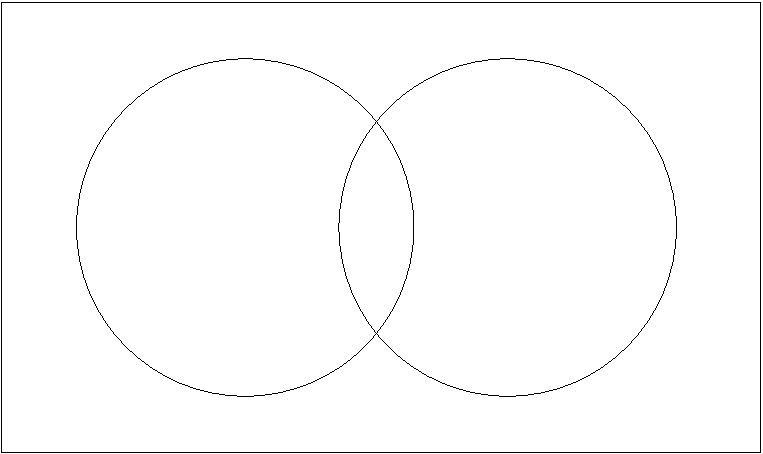
\includegraphics{figures/first_Venn.pdf}%
\end{picture}%
\setlength{\unitlength}{3947sp}%
%
\begingroup\makeatletter\ifx\SetFigFont\undefined%
\gdef\SetFigFont#1#2#3#4#5{%
  \reset@font\fontsize{#1}{#2pt}%
  \fontfamily{#3}\fontseries{#4}\fontshape{#5}%
  \selectfont}%
\fi\endgroup%
\begin{picture}(6099,3624)(1189,-3673)
\put(2326,-1036){\makebox(0,0)[lb]{\smash{{\SetFigFont{12}{14.4}{\familydefault}{\mddefault}{\updefault}{\color[rgb]{0,0,0}A}%
}}}}
\put(6001,-1036){\makebox(0,0)[lb]{\smash{{\SetFigFont{12}{14.4}{\familydefault}{\mddefault}{\updefault}{\color[rgb]{0,0,0}B}%
}}}}
\put(1276,-286){\makebox(0,0)[lb]{\smash{{\SetFigFont{12}{14.4}{\familydefault}{\mddefault}{\updefault}{\color[rgb]{0,0,0}U}%
}}}}
\end{picture}%


\vspace{.1in}

In a Venn diagram the 
\index{universe of discourse}universe of discourse is normally drawn as
a rectangular region inside of which all the action occurs.  Each
set in a Venn diagram is depicted by drawing a simple closed curve -- 
typically a circle, but not necessarily!  For instance, if you
want to draw a Venn diagram that shows all the possible intersections
among four sets, you'll find it's impossible with (only) circles.

\vspace{.1in}

\begin{picture}(0,0)%
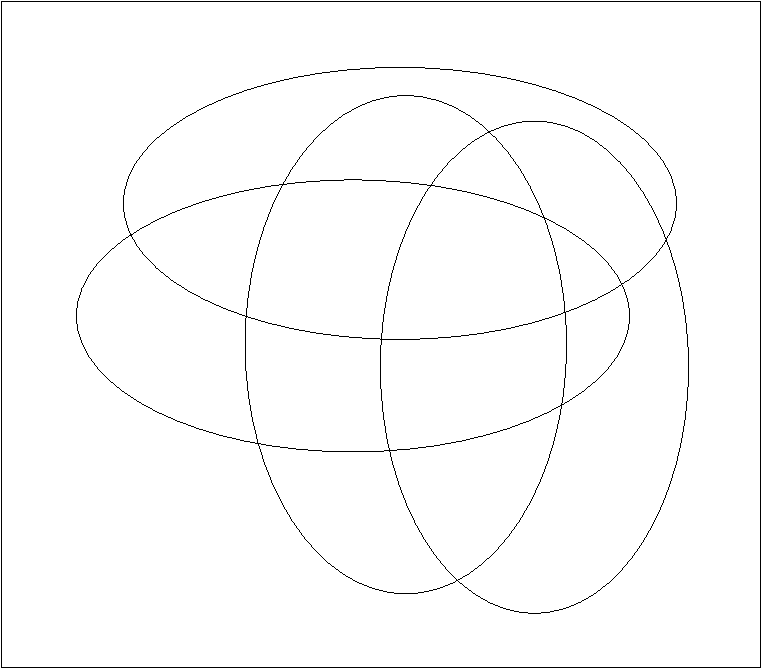
\includegraphics{figures/4set_Venn.pdf}%
\end{picture}%
\setlength{\unitlength}{3947sp}%
%
\begingroup\makeatletter\ifx\SetFigFont\undefined%
\gdef\SetFigFont#1#2#3#4#5{%
  \reset@font\fontsize{#1}{#2pt}%
  \fontfamily{#3}\fontseries{#4}\fontshape{#5}%
  \selectfont}%
\fi\endgroup%
\begin{picture}(6099,5349)(1189,-5398)
\put(1276,-286){\makebox(0,0)[lb]{\smash{{\SetFigFont{12}{14.4}{\familydefault}{\mddefault}{\updefault}{\color[rgb]{0,0,0}U}%
}}}}
\put(2551,-1261){\makebox(0,0)[lb]{\smash{{\SetFigFont{12}{14.4}{\familydefault}{\mddefault}{\updefault}{\color[rgb]{0,0,0}A}%
}}}}
\put(3976,-4636){\makebox(0,0)[lb]{\smash{{\SetFigFont{12}{14.4}{\familydefault}{\mddefault}{\updefault}{\color[rgb]{0,0,0}C}%
}}}}
\put(6001,-4561){\makebox(0,0)[lb]{\smash{{\SetFigFont{12}{14.4}{\familydefault}{\mddefault}{\updefault}{\color[rgb]{0,0,0}D}%
}}}}
\put(2026,-2911){\makebox(0,0)[lb]{\smash{{\SetFigFont{12}{14.4}{\familydefault}{\mddefault}{\updefault}{\color[rgb]{0,0,0}B}%
}}}}
\end{picture}%


\vspace{.1in}

\begin{exer}
Verify that the diagram above has regions representing all 16 possible
intersections of 4 sets.
\end{exer}

There is a certain ``zen'' to Venn diagrams that must be internalized,
but once you have done so they can be used to think very effectively
about the relationships between sets.  The main deal is that the points
inside of one of the simple closed curves are not necessarily in the set --
only \emph{some} of the points inside a simple closed curve are in the
set, and we don't know precisely where they are!  The various simple closed 
curves in a Venn diagram divide the universe up into a bunch of regions.
It might be best to think of these regions as fenced-in areas in which
the elements of a set mill about, much like domesticated animals 
in their pens.
One of our main tools in working with Venn diagrams is to deduce that
certain of these regions don't contain any elements -- we then mark that
region with the emptyset symbol ($\emptyset$). 

Here is a small example of a finite universe.

\vspace{.1in}

\begin{picture}(0,0)%
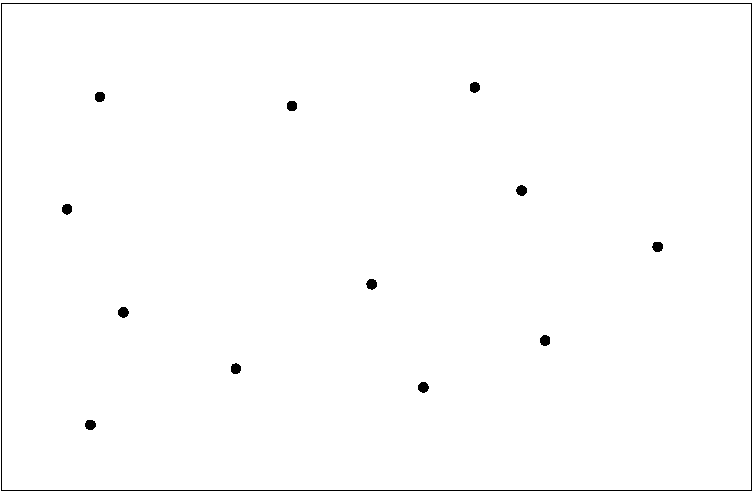
\includegraphics{figures/silly_universe.pdf}%
\end{picture}%
\setlength{\unitlength}{3947sp}%
%
\begingroup\makeatletter\ifx\SetFigFont\undefined%
\gdef\SetFigFont#1#2#3#4#5{%
  \reset@font\fontsize{#1}{#2pt}%
  \fontfamily{#3}\fontseries{#4}\fontshape{#5}%
  \selectfont}%
\fi\endgroup%
\begin{picture}(6024,3924)(1189,-4273)
\put(2101,-1036){\makebox(0,0)[lb]{\smash{{\SetFigFont{12}{14.4}{\familydefault}{\mddefault}{\updefault}{\color[rgb]{0,0,0}Mr. Ed}%
}}}}
\put(1801,-1936){\makebox(0,0)[lb]{\smash{{\SetFigFont{12}{14.4}{\familydefault}{\mddefault}{\updefault}{\color[rgb]{0,0,0}Shadowfax}%
}}}}
\put(2251,-2761){\makebox(0,0)[lb]{\smash{{\SetFigFont{12}{14.4}{\familydefault}{\mddefault}{\updefault}{\color[rgb]{0,0,0}Silver}%
}}}}
\put(2026,-3661){\makebox(0,0)[lb]{\smash{{\SetFigFont{12}{14.4}{\familydefault}{\mddefault}{\updefault}{\color[rgb]{0,0,0}Secretariat}%
}}}}
\put(3151,-3211){\makebox(0,0)[lb]{\smash{{\SetFigFont{12}{14.4}{\familydefault}{\mddefault}{\updefault}{\color[rgb]{0,0,0}Misty}%
}}}}
\put(3601,-1111){\makebox(0,0)[lb]{\smash{{\SetFigFont{12}{14.4}{\familydefault}{\mddefault}{\updefault}{\color[rgb]{0,0,0}Black Beauty}%
}}}}
\put(4201,-2536){\makebox(0,0)[lb]{\smash{{\SetFigFont{12}{14.4}{\familydefault}{\mddefault}{\updefault}{\color[rgb]{0,0,0}Heckle}%
}}}}
\put(5101,-961){\makebox(0,0)[lb]{\smash{{\SetFigFont{12}{14.4}{\familydefault}{\mddefault}{\updefault}{\color[rgb]{0,0,0}Donald Duck}%
}}}}
\put(4651,-3436){\makebox(0,0)[lb]{\smash{{\SetFigFont{12}{14.4}{\familydefault}{\mddefault}{\updefault}{\color[rgb]{0,0,0}Wile E. Coyote}%
}}}}
\put(5626,-2986){\makebox(0,0)[lb]{\smash{{\SetFigFont{12}{14.4}{\familydefault}{\mddefault}{\updefault}{\color[rgb]{0,0,0}Tweety Bird}%
}}}}
\put(6526,-2236){\makebox(0,0)[lb]{\smash{{\SetFigFont{12}{14.4}{\familydefault}{\mddefault}{\updefault}{\color[rgb]{0,0,0}Ren}%
}}}}
\put(5476,-1786){\makebox(0,0)[lb]{\smash{{\SetFigFont{12}{14.4}{\familydefault}{\mddefault}{\updefault}{\color[rgb]{0,0,0}Snowball}%
}}}}
\end{picture}%


\vspace{.1in}

\noindent And here is the same universe with some Jordan curves 
used to encircle two subsets.

\vspace{.1in}

\begin{picture}(0,0)%
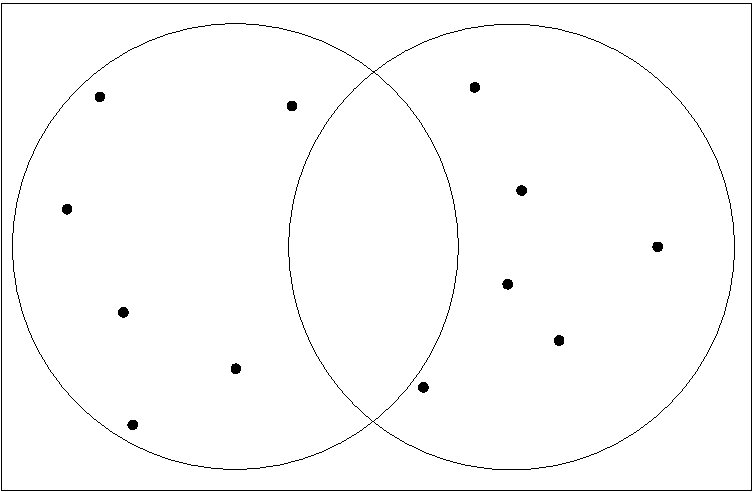
\includegraphics{./silly_w_sets.pdf}%
\end{picture}%
\setlength{\unitlength}{3947sp}%
%
\begingroup\makeatletter\ifx\SetFigFont\undefined%
\gdef\SetFigFont#1#2#3#4#5{%
  \reset@font\fontsize{#1}{#2pt}%
  \fontfamily{#3}\fontseries{#4}\fontshape{#5}%
  \selectfont}%
\fi\endgroup%
\begin{picture}(6024,3924)(1189,-4273)
\put(2101,-1036){\makebox(0,0)[lb]{\smash{{\SetFigFont{12}{14.4}{\familydefault}{\mddefault}{\updefault}{\color[rgb]{0,0,0}Mr. Ed}%
}}}}
\put(1801,-1936){\makebox(0,0)[lb]{\smash{{\SetFigFont{12}{14.4}{\familydefault}{\mddefault}{\updefault}{\color[rgb]{0,0,0}Shadowfax}%
}}}}
\put(2251,-2761){\makebox(0,0)[lb]{\smash{{\SetFigFont{12}{14.4}{\familydefault}{\mddefault}{\updefault}{\color[rgb]{0,0,0}Silver}%
}}}}
\put(3151,-3211){\makebox(0,0)[lb]{\smash{{\SetFigFont{12}{14.4}{\familydefault}{\mddefault}{\updefault}{\color[rgb]{0,0,0}Misty}%
}}}}
\put(3601,-1111){\makebox(0,0)[lb]{\smash{{\SetFigFont{12}{14.4}{\familydefault}{\mddefault}{\updefault}{\color[rgb]{0,0,0}Black Beauty}%
}}}}
\put(5101,-961){\makebox(0,0)[lb]{\smash{{\SetFigFont{12}{14.4}{\familydefault}{\mddefault}{\updefault}{\color[rgb]{0,0,0}Donald Duck}%
}}}}
\put(5326,-2536){\makebox(0,0)[lb]{\smash{{\SetFigFont{12}{14.4}{\familydefault}{\mddefault}{\updefault}{\color[rgb]{0,0,0}Heckle}%
}}}}
\put(2326,-3661){\makebox(0,0)[lb]{\smash{{\SetFigFont{12}{14.4}{\familydefault}{\mddefault}{\updefault}{\color[rgb]{0,0,0}Secretariat}%
}}}}
\put(5476,-1786){\makebox(0,0)[lb]{\smash{{\SetFigFont{12}{14.4}{\familydefault}{\mddefault}{\updefault}{\color[rgb]{0,0,0}Snowball}%
}}}}
\put(4651,-3361){\makebox(0,0)[lb]{\smash{{\SetFigFont{12}{14.4}{\familydefault}{\mddefault}{\updefault}{\color[rgb]{0,0,0}Wile E. Coyote}%
}}}}
\put(6526,-2236){\makebox(0,0)[lb]{\smash{{\SetFigFont{12}{14.4}{\familydefault}{\mddefault}{\updefault}{\color[rgb]{0,0,0}Ren}%
}}}}
\put(1501,-3511){\makebox(0,0)[lb]{\smash{{\SetFigFont{12}{14.4}{\familydefault}{\mddefault}{\updefault}{\color[rgb]{0,0,0}H}%
}}}}
\put(6601,-3661){\makebox(0,0)[lb]{\smash{{\SetFigFont{12}{14.4}{\familydefault}{\mddefault}{\updefault}{\color[rgb]{0,0,0}C}%
}}}}
\put(5701,-2986){\makebox(0,0)[lb]{\smash{{\SetFigFont{12}{14.4}{\familydefault}{\mddefault}{\updefault}{\color[rgb]{0,0,0}Tweety Bird}%
}}}}
\end{picture}%


\vspace{.1in}

This picture might lead us to think that the set of cartoon characters
and the set of horses are disjoint, so we thought it would be nice
to add one more element to our universe in order to dispel that notion.

\vspace{.1in}

\begin{picture}(0,0)%
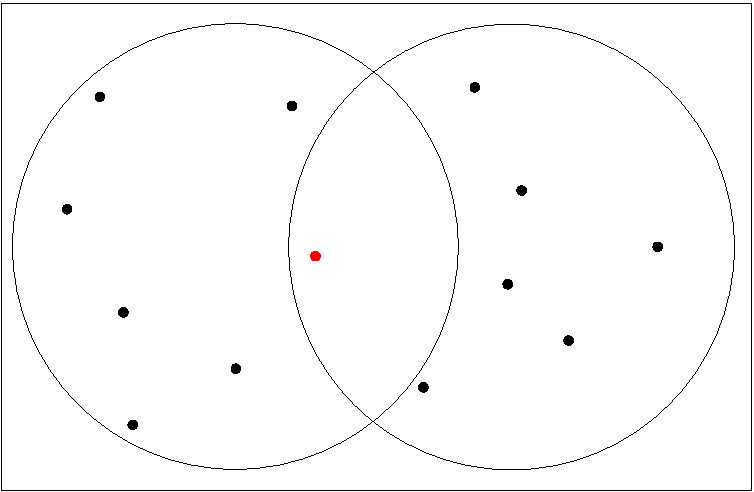
\includegraphics{./silly_w_counter_ex.pdf}%
\end{picture}%
\setlength{\unitlength}{3947sp}%
%
\begingroup\makeatletter\ifx\SetFigFont\undefined%
\gdef\SetFigFont#1#2#3#4#5{%
  \reset@font\fontsize{#1}{#2pt}%
  \fontfamily{#3}\fontseries{#4}\fontshape{#5}%
  \selectfont}%
\fi\endgroup%
\begin{picture}(6024,3924)(1189,-4273)
\put(2101,-1036){\makebox(0,0)[lb]{\smash{{\SetFigFont{12}{14.4}{\familydefault}{\mddefault}{\updefault}{\color[rgb]{0,0,0}Mr. Ed}%
}}}}
\put(1801,-1936){\makebox(0,0)[lb]{\smash{{\SetFigFont{12}{14.4}{\familydefault}{\mddefault}{\updefault}{\color[rgb]{0,0,0}Shadowfax}%
}}}}
\put(2251,-2761){\makebox(0,0)[lb]{\smash{{\SetFigFont{12}{14.4}{\familydefault}{\mddefault}{\updefault}{\color[rgb]{0,0,0}Silver}%
}}}}
\put(3151,-3211){\makebox(0,0)[lb]{\smash{{\SetFigFont{12}{14.4}{\familydefault}{\mddefault}{\updefault}{\color[rgb]{0,0,0}Misty}%
}}}}
\put(3601,-1111){\makebox(0,0)[lb]{\smash{{\SetFigFont{12}{14.4}{\familydefault}{\mddefault}{\updefault}{\color[rgb]{0,0,0}Black Beauty}%
}}}}
\put(5101,-961){\makebox(0,0)[lb]{\smash{{\SetFigFont{12}{14.4}{\familydefault}{\mddefault}{\updefault}{\color[rgb]{0,0,0}Donald Duck}%
}}}}
\put(5326,-2536){\makebox(0,0)[lb]{\smash{{\SetFigFont{12}{14.4}{\familydefault}{\mddefault}{\updefault}{\color[rgb]{0,0,0}Heckle}%
}}}}
\put(2326,-3661){\makebox(0,0)[lb]{\smash{{\SetFigFont{12}{14.4}{\familydefault}{\mddefault}{\updefault}{\color[rgb]{0,0,0}Secretariat}%
}}}}
\put(5476,-1786){\makebox(0,0)[lb]{\smash{{\SetFigFont{12}{14.4}{\familydefault}{\mddefault}{\updefault}{\color[rgb]{0,0,0}Snowball}%
}}}}
\put(4651,-3361){\makebox(0,0)[lb]{\smash{{\SetFigFont{12}{14.4}{\familydefault}{\mddefault}{\updefault}{\color[rgb]{0,0,0}Wile E. Coyote}%
}}}}
\put(6526,-2236){\makebox(0,0)[lb]{\smash{{\SetFigFont{12}{14.4}{\familydefault}{\mddefault}{\updefault}{\color[rgb]{0,0,0}Ren}%
}}}}
\put(1501,-3511){\makebox(0,0)[lb]{\smash{{\SetFigFont{12}{14.4}{\familydefault}{\mddefault}{\updefault}{\color[rgb]{0,0,0}H}%
}}}}
\put(6601,-3661){\makebox(0,0)[lb]{\smash{{\SetFigFont{12}{14.4}{\familydefault}{\mddefault}{\updefault}{\color[rgb]{0,0,0}C}%
}}}}
\put(3826,-2311){\makebox(0,0)[lb]{\smash{{\SetFigFont{12}{14.4}{\familydefault}{\mddefault}{\updefault}{\color[rgb]{1,0,0}Night Mare}%
}}}}
\put(5776,-2986){\makebox(0,0)[lb]{\smash{{\SetFigFont{12}{14.4}{\familydefault}{\mddefault}{\updefault}{\color[rgb]{0,0,0}Tweety Bird}%
}}}}
\end{picture}%


\vspace{.1in}


Suppose we have two sets $A$ and $B$ and we're interested
in proving that $B \subseteq A$.  The job is done if we can show that
all of $B$'s elements are actually in the eye-shaped region that represents
the intersection $A \cap B$.  It's equivalent if we can show that the
region marked with $\emptyset$ in the following diagram is actually empty.

\vspace{.1in}

\begin{picture}(0,0)%
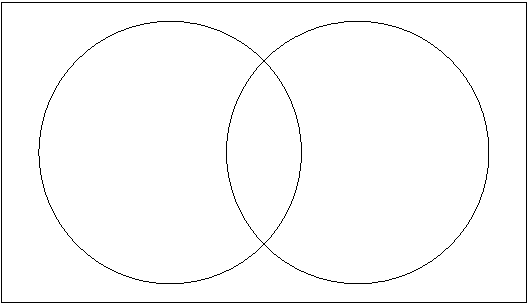
\includegraphics{./Venn_showing_implies.pdf}%
\end{picture}%
\setlength{\unitlength}{3947sp}%
%
\begingroup\makeatletter\ifx\SetFigFont\undefined%
\gdef\SetFigFont#1#2#3#4#5{%
  \reset@font\fontsize{#1}{#2pt}%
  \fontfamily{#3}\fontseries{#4}\fontshape{#5}%
  \selectfont}%
\fi\endgroup%
\begin{picture}(4224,2424)(2389,-2773)
\put(2926,-736){\makebox(0,0)[lb]{\smash{{\SetFigFont{12}{14.4}{\familydefault}{\mddefault}{\updefault}{\color[rgb]{0,0,0}A}%
}}}}
\put(6001,-736){\makebox(0,0)[lb]{\smash{{\SetFigFont{12}{14.4}{\familydefault}{\mddefault}{\updefault}{\color[rgb]{0,0,0}B}%
}}}}
\put(5251,-1561){\makebox(0,0)[lb]{\smash{{\SetFigFont{12}{14.4}{\familydefault}{\mddefault}{\updefault}{\color[rgb]{0,0,0}$\emptyset$}%
}}}}
\end{picture}%


\vspace{.1in}

Let's put all this together.  The inclusion $B \subseteq A$ corresponds
to the logical sentence $M_B \implies M_A$.  We know that implications
are equivalent to OR statements, so $M_B \implies M_A \, \cong \, 
{\lnot}M_B \lor M_A$.  The notion that the region we've 
indicated above is empty is written as $\overline{A} \cap B \, = \, \emptyset$,
in logical terms this is ${\lnot}M_A \land M_B \, \cong \, c$.  
Finally, we apply DeMorgan's law and a commutation to get 
${\lnot}M_B \lor M_A \, \cong \, t$.  You should take note of the 
convention that when you see a logical sentence just written on the 
page (as is the case with $M_B \implies M_A$ in the first sentence
of this paragraph) what's being asserted is that the sentence is 
\emph{universally true}.
Thus, writing $M_B \implies M_A$ is the same thing as writing 
$M_B \implies M_A \, \cong \, t$.

One can use information that is known \emph{a priori} when 
drawing a Venn diagram.  For instance if two sets are known 
to be disjoint, or if one is known to be contained in the other,
we can draw Venn diagrams like the following.

\vspace{.1in}

\begin{picture}(0,0)%
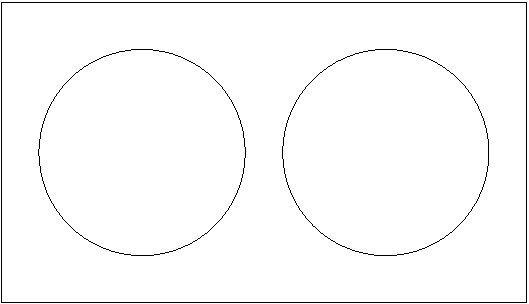
\includegraphics{figures/disjoint_Venn.pdf}%
\end{picture}%
\setlength{\unitlength}{3947sp}%
%
\begingroup\makeatletter\ifx\SetFigFont\undefined%
\gdef\SetFigFont#1#2#3#4#5{%
  \reset@font\fontsize{#1}{#2pt}%
  \fontfamily{#3}\fontseries{#4}\fontshape{#5}%
  \selectfont}%
\fi\endgroup%
\begin{picture}(4224,2424)(2389,-2773)
\put(2926,-736){\makebox(0,0)[lb]{\smash{{\SetFigFont{12}{14.4}{\familydefault}{\mddefault}{\updefault}{\color[rgb]{0,0,0}A}%
}}}}
\put(6001,-736){\makebox(0,0)[lb]{\smash{{\SetFigFont{12}{14.4}{\familydefault}{\mddefault}{\updefault}{\color[rgb]{0,0,0}B}%
}}}}
\end{picture}%


\vspace{.2in}

\begin{picture}(0,0)%
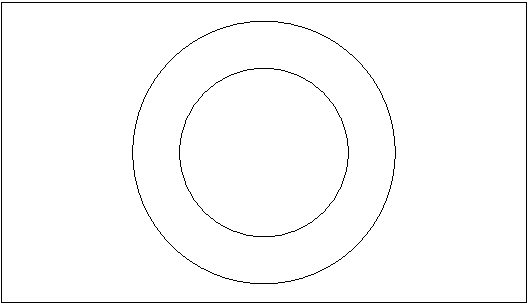
\includegraphics{figures/containment_Venn.pdf}%
\end{picture}%
\setlength{\unitlength}{3947sp}%
%
\begingroup\makeatletter\ifx\SetFigFont\undefined%
\gdef\SetFigFont#1#2#3#4#5{%
  \reset@font\fontsize{#1}{#2pt}%
  \fontfamily{#3}\fontseries{#4}\fontshape{#5}%
  \selectfont}%
\fi\endgroup%
\begin{picture}(4224,2424)(2389,-2773)
\put(3676,-736){\makebox(0,0)[lb]{\smash{{\SetFigFont{12}{14.4}{\familydefault}{\mddefault}{\updefault}{\color[rgb]{0,0,0}A}%
}}}}
\put(4726,-1186){\makebox(0,0)[lb]{\smash{{\SetFigFont{12}{14.4}{\familydefault}{\mddefault}{\updefault}{\color[rgb]{0,0,0}B}%
}}}}
\end{picture}%


\vspace{.1in}

However, both of these situations can also be dealt with
by working with Venn diagrams in which the sets are in 
\index{general position} \emph{general position} -- which
in this situation means that every possible intersection is
shown -- and then marking any empty regions with $\emptyset$.

\begin{exer}
On a Venn diagram for two sets in general position, indicate
the empty regions when
\begin{itemize}
\item[a)] The sets are disjoint.
\item[b)] $A$ is contained in $B$.
\end{itemize}

\begin{picture}(0,0)%
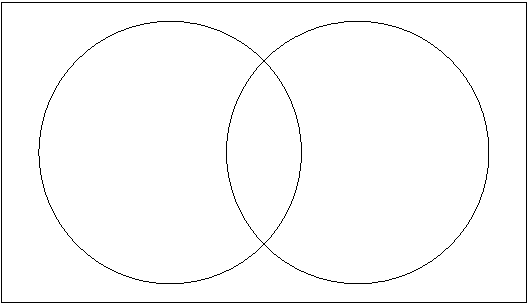
\includegraphics{./general_Venn.pdf}%
\end{picture}%
\setlength{\unitlength}{3947sp}%
%
\begingroup\makeatletter\ifx\SetFigFont\undefined%
\gdef\SetFigFont#1#2#3#4#5{%
  \reset@font\fontsize{#1}{#2pt}%
  \fontfamily{#3}\fontseries{#4}\fontshape{#5}%
  \selectfont}%
\fi\endgroup%
\begin{picture}(4224,2424)(2389,-2773)
\put(2926,-736){\makebox(0,0)[lb]{\smash{{\SetFigFont{12}{14.4}{\familydefault}{\mddefault}{\updefault}{\color[rgb]{0,0,0}A}%
}}}}
\put(6001,-736){\makebox(0,0)[lb]{\smash{{\SetFigFont{12}{14.4}{\familydefault}{\mddefault}{\updefault}{\color[rgb]{0,0,0}B}%
}}}}
\end{picture}%

\end{exer}

There is a connection, perhaps obvious, between the regions we
see in a Venn diagram with sets in general position and the recognizers
we studied in the section on digital logic circuits.  In fact both
of these topics have to do with \index{disjunctive normal form}\emph{disjunctive normal form}.  In a Venn diagram with $k$ sets, we are seeing the universe
of discourse broken up into the union of $2^k$ regions each of which 
corresponds to an intersection of either one of the sets or its complement.
An arbitrary expression involving set-theoretic symbols and these $k$ sets
is true in certain of these $2^k$ regions and false in the others.  
We have put the arbitrary expression in disjunctive normal form when
we express it as a union of the intersections that describe those regions.

\vspace{.1in}

\begin{picture}(0,0)%
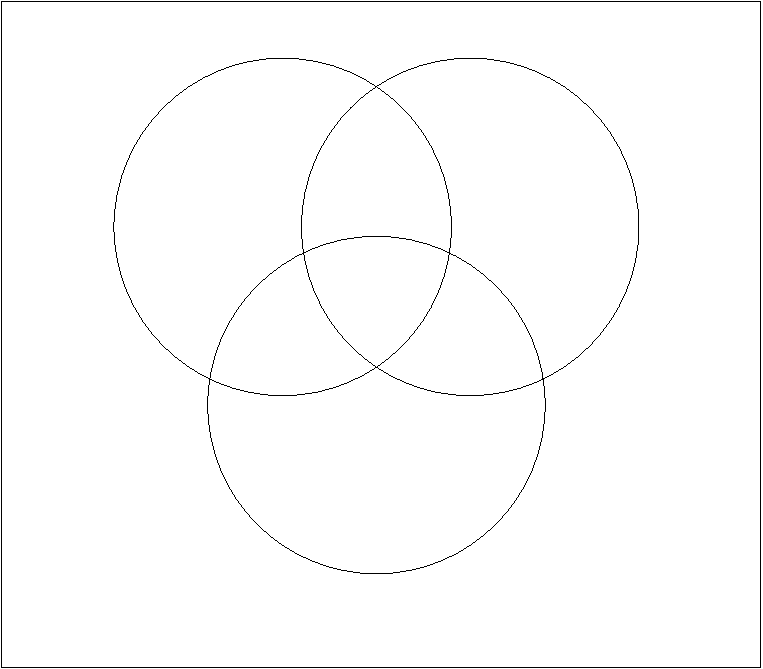
\includegraphics{figures/3set_Venn_gen_pos.pdf}%
\end{picture}%
\setlength{\unitlength}{3947sp}%
%
\begingroup\makeatletter\ifx\SetFigFont\undefined%
\gdef\SetFigFont#1#2#3#4#5{%
  \reset@font\fontsize{#1}{#2pt}%
  \fontfamily{#3}\fontseries{#4}\fontshape{#5}%
  \selectfont}%
\fi\endgroup%
\begin{picture}(6099,5349)(1189,-5398)
\put(1276,-286){\makebox(0,0)[lb]{\smash{{\SetFigFont{12}{14.4}{\familydefault}{\mddefault}{\updefault}{\color[rgb]{0,0,0}$U$}%
}}}}
\put(2326,-1486){\makebox(0,0)[lb]{\smash{{\SetFigFont{12}{14.4}{\familydefault}{\mddefault}{\updefault}{\color[rgb]{0,0,0}$A\cap\overline{B}\cap\overline{C}$}%
}}}}
\put(3751,-1711){\makebox(0,0)[lb]{\smash{{\SetFigFont{12}{14.4}{\familydefault}{\mddefault}{\updefault}{\color[rgb]{0,0,0}$A\cap B\cap\overline{C}$}%
}}}}
\put(3751,-2311){\makebox(0,0)[lb]{\smash{{\SetFigFont{12}{14.4}{\familydefault}{\mddefault}{\updefault}{\color[rgb]{0,0,0}$A\cap B\cap C$}%
}}}}
\put(3001,-2986){\makebox(0,0)[lb]{\smash{{\SetFigFont{12}{14.4}{\familydefault}{\mddefault}{\updefault}{\color[rgb]{0,0,0}$A\cap\overline{B}\cap C$}%
}}}}
\put(1351,-4561){\makebox(0,0)[lb]{\smash{{\SetFigFont{12}{14.4}{\familydefault}{\mddefault}{\updefault}{\color[rgb]{0,0,0}$\overline{A}\cap\overline{B}\cap\overline{C}$}%
}}}}
\put(2326,-811){\makebox(0,0)[lb]{\smash{{\SetFigFont{12}{14.4}{\familydefault}{\mddefault}{\updefault}{\color[rgb]{0,0,0}$A$}%
}}}}
\put(6001,-811){\makebox(0,0)[lb]{\smash{{\SetFigFont{12}{14.4}{\familydefault}{\mddefault}{\updefault}{\color[rgb]{0,0,0}$B$}%
}}}}
\put(4426,-4861){\makebox(0,0)[lb]{\smash{{\SetFigFont{12}{14.4}{\familydefault}{\mddefault}{\updefault}{\color[rgb]{0,0,0}$C$}%
}}}}
\put(4501,-2986){\makebox(0,0)[lb]{\smash{{\SetFigFont{12}{14.4}{\familydefault}{\mddefault}{\updefault}{\color[rgb]{0,0,0}$\overline{A}\cap B\cap C$}%
}}}}
\put(3751,-3736){\makebox(0,0)[lb]{\smash{{\SetFigFont{12}{14.4}{\familydefault}{\mddefault}{\updefault}{\color[rgb]{0,0,0}$\overline{A}\cap\overline{B}\cap C$}%
}}}}
\put(4951,-1486){\makebox(0,0)[lb]{\smash{{\SetFigFont{12}{14.4}{\familydefault}{\mddefault}{\updefault}{\color[rgb]{0,0,0}$\overline{A}\cap B\cap\overline{C}$}%
}}}}
\end{picture}%

 

\clearpage 

\noindent{\large \bf Exercises --- \thesection\ }

\begin{enumerate}
\item  Venn diagrams are usually made using simple closed curves 
with no further restrictions.  Try creating Venn diagrams for 3, 4 and
5 sets (in general position) using rectangular simple closed curves.

\hint{I found it easier to experiment by making my drawings on graph paper.  I never did  
manage to draw the $5$ set Venn diagram with just rectangles\ldots probably just a lack of persistence.}

\item  We call a curve \emph{rectilinear} if it is made
of line segments that meet at right angles.  Use rectilinear
simple closed curves to create a Venn diagram for 5 sets.

\hint{Of course, rectangles are rectilinear, so one could use the solution from the previous
problem (if, unlike me, you were persistant enough to find it).  Otherwise, 
start with the $4$ set diagram made with rectangles and use your $5$th (rectilinear) curve to split
each region into $2$ -- don't forget to split the region on the outside too.}

\item  Argue as to why rectilinear curves will suffice to build
any Venn diagram.

\hint{Fortunately the instructions don't say to {\em prove} that rectilinear curves will always
suffice, so we can be less rigorous.  Try to argue as to why it will alway be possible to add one more rectilinear curve to an existing Venn diagram and split every region into two.}

\item  Find the disjunctive normal form of $A \cap (B \cup C)$.

\hint{ $ (A \cap B \cap \overline{C}) \cup (A \cap \overline{B} \cap C) $ }

\item  Find the disjunctive normal form of $(A \triangle B) \triangle C$

\hint{It is $(A \cap \overline{B} \cap \overline{C}) \cup (\overline{A} \cap B \cap \overline{C}) \cup (\overline{A} \cap \overline{B} \cap C)$.  Now find the disjunctive normal form of 
$A \triangle (B \triangle C)$.}

\item The prototypes for the \emph{modus ponens} and \emph{modus tollens}
argument forms are the following:

\begin{tabular}{lcl}
\begin{minipage}{.3\textwidth}All men are mortal. \newline %
Socrates is a man. \newline
Therefore Socrates is mortal.\end{minipage} & \rule{16pt}{0pt} and \rule{16pt}{0pt} & %
 \begin{minipage}{.3\textwidth}All men are mortal. \newline %
Zeus is not mortal. \newline
Therefore Zeus is not a man.\end{minipage}
\end{tabular}

Illustrate these arguments using Venn diagrams.

\hint{The statement ``All men are mortal'' would be interpreted on a Venn diagram by showing the
set of ``All men'' as being entirely contained within the set of ``mortal beings.''   Socrates is an 
element of the inner set.  Zeus, on the other hand, lies outside of the outer set.}
 
\item Use Venn diagrams to convince yourself of the validity of
the following containment statement

\[ (A \cap B) \cup (C \cap D) \; \subseteq \; (A \cup C) \cap (B \cup D).\]

Now prove it!
 
\hint{Obviously we'll need one of the $4$-set Venn diagrams.}
 
\item Use Venn diagrams to show that the following set equivalence is false.

\[ (A \cup B) \cap (C \cup D) \; = \; (A \cup C) \cap (B \cup D) \]

\hint{After constructing Venn diagrams for both sets you should be able to see that there
are $4$ regions where they differ.  One is $A \cap B \cap \overline{C} \cap \overline{D}$.
What are the other three?}

\end{enumerate}



%% Emacs customization
%% 
%% Local Variables: ***
%% TeX-master: "GIAM-hw.tex" ***
%% comment-column:0 ***
%% comment-start: "%% "  ***
%% comment-end:"***" ***
%% End: ***



\newpage

\section{Russell's Paradox}
\label{sec:russell}

There is no Nobel prize category for mathematics.\footnote{There are prizes
considered equivalent to the Nobel in stature -- the Fields Medal, awarded every four years by the International Mathematical Union to up to four mathematical researchers under the age of forty, and the Abel Prize, awarded annually by the King of Norway.}   Alfred Nobel's will
called for the awarding of annual prizes in physics, chemistry, physiology 
or medicine, literature, and peace.  Later, the 
``Bank of Sweden Prize in Economic Sciences in Memory of Alfred Nobel'' 
was created and certainly several mathematicians have won what is 
improperly known as the Nobel prize in Economics.  But, there is no 
Nobel prize in Mathematics per se.  There is an interesting urban myth that
purports to explain this lapse: Alfred Nobel's wife either left him for, or
had an affair with a mathematician --- so Nobel, the inventor of dynamite
and an immensely wealthy and powerful man, when he decided to endow 
a set of annual prizes for ``those who, during the preceding year, shall have conferred the greatest benefit on mankind'' pointedly left out mathematicians.

One major flaw in this theory is that Nobel was never married.

In all likelihood, Nobel simply didn't view mathematics as a field
which provides benefits for mankind --- at least not directly. 
The broadest division within mathematics is between the ``pure''
and ``applied'' branches.  Just precisely where the dividing line
between these spheres lies is a matter of opinion, but it can be
argued that it is so far to one side that one may as well call an
applied mathematician a physicist 
(or chemist, or biologist, or economist, or \ldots).  One thing is
clear, Nobel believed to a certain extent in the utilitarian ethos.
The value of a thing (or a person) is determined by how useful it is (or they 
are), which makes it interesting that one of the few mathematicians
to win a Nobel prize was Bertrand Russell (the 1950 prize in Literature
 ``in recognition of his varied and significant writings in which he 
champions humanitarian ideals and freedom of thought''). 
 
Bertrand Russell was one of the twentieth century's most colorful
intellectuals.  He helped revolutionize the foundations of mathematics,
but was perhaps better known as a philosopher.  It's hard to conceive 
of \emph{anyone} who would characterize Russell as an applied mathematician!

Russell was an ardent anti-war and anti-nuclear activist.  He achieved a
status (shared with Albert Einstein, but very few others) as an eminent
scientist who was also a powerful moral authority.  Russell's mathematical
work was of a very abstruse foundational sort; he was concerned with
the idea of reducing all mathematical thought to Logic and Set theory.

In the beginning of our investigations into Set theory we mentioned 
that the notion of a ``set of all sets'' leads to something paradoxical.
Now we're ready to look more closely into that remark and hopefully 
gain an understanding of Russell's paradox.

By this point you should be okay with the notion of a set that 
contains other sets, but would it be okay for a set to contain
\emph{itself}?  That is, would it make sense to have a set 
defined by

\[ A = \{ 1, 2, A \}? \]

\noindent The set $A$ has three elements, $1$, $2$ and itself.  So we
could write

\[ A = \{ 1, 2, \{ 1, 2, A \} \}, \]
 
\noindent and then

\[ A = \{ 1, 2, \{ 1, 2, \{ 1, 2, A \} \} \}, \]

\noindent and then

\[ A = \{ 1, 2, \{ 1, 2, \{ 1, 2, \{ 1, 2, A \} \} \} \}, \]
  
\noindent et cetera.

This obviously seems like a problem.  Indeed, often paradoxes seem to
be caused by self-reference of this sort.  Consider 

\begin{center} 
\framebox[1.1\width]{The sentence in this box is false.}  
\end{center}

So a reasonable alternative
is to ``do'' math among the sets that don't exhibit this particular
pathology.  

Thus, inside the set of all sets we are singling out a particular subset
that consists of sets which don't contain themselves.  

\[ {\mathcal S} = \{ A \suchthat \; A \,\mbox{is a set} \; \land \; A \notin A \} \]

Now within the universal set we're working in (the set of all sets) there
are only two possibilities: a given set is either in ${\mathcal S}$ or
it is in its complement $\overline{\mathcal S}$.  Russell's paradox 
comes about when we try to decide which of these alternatives pertains
to ${\mathcal S}$ itself, the problem is that each alternative leads us 
to the other!

If we assume that ${\mathcal S} \in {\mathcal S}$, then it must be the 
case that ${\mathcal S}$ satisfies the membership criterion for ${\mathcal S}$.
Thus, ${\mathcal S} \notin {\mathcal S}$.

On the other hand, if we assume that ${\mathcal S} \notin {\mathcal S}$,
then we see that ${\mathcal S}$ does indeed satisfy the membership criterion for ${\mathcal S}$.  Thus ${\mathcal S} \in {\mathcal S}$.

Russell himself developed a workaround for the paradox which
bears his name.  Together with Alfred North Whitehead he published
a 3 volume work entitled \emph{Principia Mathematica}\footnote{Isaac Newton
also published a 3 volume work which is often cited by this same title,
\emph{Philosophiae Naturalis Principia Mathematica}.} \cite{PM}.  
In the Principia, Whitehead and Russell develop a system known as 
\emph{type theory} which sets forth principles for avoiding problems
like Russell's paradox.  Basically, a set and its elements are of
different ``types'' and so the notion of a set being contained in itself
(as an element) is disallowed.

\clearpage 

\noindent{\large \bf Exercises --- \thesection\ }

\begin{enumerate}
\item Verify that $(A \implies {\lnot}A) \land ({\lnot}A \implies A)$
is a logical contradiction in two ways:  by filling out a truth table and 
using the laws of logical equivalence.

\hint{In order to get started on this you'll need to convert the conditionals into equivalent
disjunctions.  Recall that $X \implies Y \; \equiv \; {\lnot}X \lor Y$.}

\item One way out of Russell's paradox is to declare that the collection
of sets that don't contain themselves as elements is not a set itself.
Explain how this circumvents the paradox. 

\hint{If it's not a set then it doesn't necessarily have to have the property that we
can be {\em sure} whether an element is in it or not.}

\end{enumerate}


%% Emacs customization
%% 
%% Local Variables: ***
%% TeX-master: "GIAM-hw.tex" ***
%% comment-column:0 ***
%% comment-start: "%% "  ***
%% comment-end:"***" ***
%% End: ***



%\newpage
%
%\renewcommand{\bibname}{References for chapter 4}
%\bibliographystyle{plain}
%\bibliography{main}

%% Emacs customization
%% 
%% Local Variables: ***
%% TeX-master: "GIAM.tex" ***
%% comment-column:0 ***
%% comment-start: "%% "  ***
%% comment-end:"***" ***
%% End: ***

